\section{Problemformulering}
Tracking af en lerdue i English Skeet (ES) vha. PTS. 
Lerduen/målet regnes i vores opstilling blot som et punkt, men ellers følges reglerne for ES \citep{ES_regler}.
Bolden bevæger sig i et 3D-rum med negligerbar luftmodstand. 

\begin{figure}[th!]
\centering
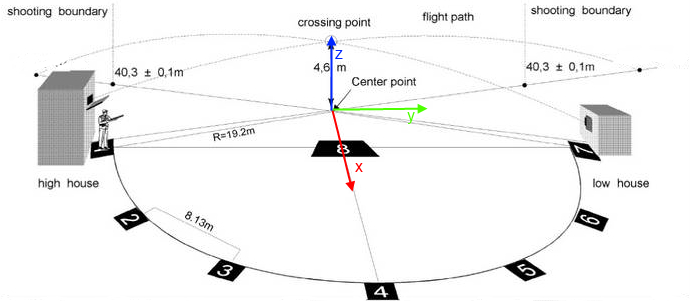
\includegraphics[width=1\textwidth]{./graphics/skeet_diagram_cropped_axes}
\caption[tekst i indholdsfortegnelsen]{figurtekst}
\label{fig:ES}
\end{figure}	
Systemets input er 60 kartesisiske koordinatsæt (x,y,z) per sekund. Hvor disse 
koordinater stammer fra er uden for projektafgrænsningen. 

Systemet dimensioneres til brug ifm. en konkurrence i ES. En skitse over 
banen ses på figur \ref{fig:ES}.
% Det kartesiske koordinatsystem har origo i halvcirklens centrum, som indtegnet nederst på figuren. 
I ES skal rammes serier af duer/mål der afskydes fra 
enten ”High House” eller ”Low House”, og med skud fra hver af de otte stationer langs 
cirkelperiferien. Dette projekt er afgrænset til et enkelt tilfælde - afskydning fra ”High-House” med PTS placeret på station 4. 

Det kartesiske koordinatsystem har origo banens centrum. Akserne er indtegnet på figur \ref{fig:ES}. PTS's origo er placeret 45 [cm] over jorden. Ved begyndelsen af applikationen er PTS stationært, med både $\phi$ og $\theta$ lig med 0. Dvs. at tilt rammen er parallel med YZ planet. 

Målets parabel er givet ved vektorfunktionen \ref{eq:pf:vektorparabel3d}

\begin{equation}
Pos\left( t \right) = 
\left( \begin{matrix} 
	x\left( t \right)  \\ 
	y\left( t \right)  \\ 
	z\left( t \right)  \end{matrix} \right) =	\left( \begin{matrix}
	32,851\cdot t-19,2 \\
	9,34\cdot t+5,5 \\
	-{ 4,91\cdot t }^{ 2 }+5,473\cdot t+3,05 
 \end{matrix} \right) 
\label{eq:pf:vektorparabel3d}
\end{equation}

Herunder er parablen vist i projekteret ned på et 
2D plan, figur \ref{fig:HH2D_para}.

Målet bliver affyret med en hastighed på 34,589 \([\frac{m}{s}]\), i en vinkel på \(9,103^{\circ}\) ift. xz-
planet. Set ovenfra bevæger målet sig som set på figur \ref{fig:para_in_xy_plane}. 
Figuren ses nedslagspunktet fra High-House, der er i alt 52 [m] startpositionen samt 
PTS placering i punktet B. 

Geværet der bruges i English Skeet har en spredning på ca. 2\degree . Systemet skal altså sigte efter målet med en nøjagtighed på $\pm 1 \degree$ før geværet affyres.
Ideelt set skal skytten skyde ca. når målet rammer toppunktet. 
Derfor skal PTS følge systemet, senest når målet når toppunktet. 
Geværet er monteret vinkelret på tilt-planet, og luftmodstand samt tyngdekraft.

Pan-rammen er begrænset til 170\degree  bevægelsesfrihed, og begrænser derved systemets maksimalt tilladte overshoot.

%
%\begin{equation}
%	T_{settling} = t_{toppunkt} = 0,557 s
%\end{equation}
%
Systemets 



\begin{figure}[h!]
\centering
%
\subfloat[Viser parablen af lerduens bane i 2D med højde som funktion af afstanden.\label{fig:HH2D_para}]{%
	\begin{tikzpicture}[scale=0.8]
	\include*{./graphics/high_house_2D_parabola}
	\end{tikzpicture}
}
\subfloat[Målets bane projekteret på xy-planet\label{fig:para_in_xy_plane}]{%
	\begin{tikzpicture}[scale=0.16]
	\include*{./graphics/parabola_in_xy_plane}
	\end{tikzpicture}
}
\caption[Målets parabel i 2 dimensioner]{Parablen i 2D}
\end{figure}



\begin{figure}[!th]
\centering
\begin{tikzpicture}[scale=2]
\include*{./graphics/3d_parabola_in_xyz_plane}
\end{tikzpicture}
\caption[tekst i indholdsfortegnelsen]{Viser målets postion med en samplefrekvens på 10 [Hz] set ovenfra. D er udgangspunktet, G er nedslagspunktet. B er placeringen af PTS.}
\label{fig:para_in_xyz_plane}
\end{figure}



\subsection{Udregning af tallene}
\label{sec:udregning_af_parabel}
\todo[inline, author=Michael]{Skal sikkert flyttes til appendix? \\ Bør omskrives lidt: Flyt origo til PTS med det samme, start med kasteparablen, find 3 variable vha. 3 datasæt, Jobs done!}


Jævnfør reglerne for ES, skal duer/mål passere target crossing point (TCS) som er 
placeret i 4,57 [m] over origo. (0 ; 0 ; 4.57). Fejlmargin for passagen er \(\pm\)0,45 [m]. 
Målene skal desuden flyve 50 - 52 [m].  High house er placeret 20,11 [m] fra TCS, i en 
højde af 3,05 [m]. 

Da luftmodstanden er negligerbar kan parablen (2. grads polynomium) findes ved at indsætte de kendte punkter. 

For at simplificere udregningerne, regnes parablen kun i 2D. Det er trivielt at tilføje den tredje, så det gøres til sidst (hvis jeg finder det relevant). 

Kasteparablen er givet ved vektorfunktionen i ligning  \ref{eq:pf:vektorparabel}.

\begin{equation}
	Pos(t) = \left( \begin{array}{c}
	x_{2D}(t) \\
	y_{2D}(t)
	\end{array}
	\right)
	= \left( \begin{array}{c}
	\cos \theta v_0 t + x_0 \\
	\sin \theta v_0 t - \frac{g}{2} t^2 + y_0
	\end{array}
	\right)
\label{eq:pf:vektorparabel}
\end{equation}

Hvor \(\theta\) er afskydningsvinklen, \(v_0\) er afskydningshastigheden, \(g\) er tyngdeacceleration og \(x_0\), \(y_0\) er begyndelsespunktet. 

For at få en parabel på formen y(x), isoleres t i x(t) med henblik på at substituere t i y(x): (\(x_0\) sættes til 0.)

\begin{equation}
t = \frac{x}{\cos \left( \theta \right) v_0}
\label{eq:pf:x(t)}
\end{equation}

Den fundne værdi for t indsættes i \(y(t)\), og udtrykket reduceres, \citep[Side. 67]{fund_of_physics}: 

\begin{align}
\begin{split}
y(t(x)) &= \sin \left( \theta \right) \frac{x}{\cos \left( \theta \right) v_0} v_0 - \frac{g}{2} \left(\frac{x}{\cos \left( \theta \right) v_0}\right)^2 + y_0 \\
y(x) &= \tan \left( \theta \right) x - \frac{gx^2}{2(\cos \left( \theta \right) v_0)^2} + y_0
\label{eq:pf:y(x(t))}
\end{split}
\end{align}

Det ses at der er 3 ubekendte i ligningen. Dog er 3 punkter kendt fra HH parablen. Det er givet i reglerne for ESS at målet affyres fra en højde på \(y_0\) = 3,05 [m], så det indsættes i formlen. 
\begin{equation}
y(x) = \tan \theta x - \frac{gx^2}{2(\cos \left( \theta \right)  v_0)^2} + 3,05
\label{eq:pf:y(x)2}
\end{equation}
Det er givet at målet skal passere TCS som er placeret i en højde på 4,57 [m], 20,11 [m] fra HH. 
Desuden skal målet bevæge sig 50 - 52 [m], i de videre beregninger 52 [m]. Det giver koordinatsættene (20,11 ; 4,57) og (52 ; 0). Vha. disse bestemmes \(\theta\) og \(v_0\) til:\footnote{Ved \(g = 9,82[m/{s}^{2]}\)}
\todo[inline, author=Michael]{Måske giver det ikke mening med alle de decimaler, da det er udregnet med g = 9,82 - men jeg ved heller ikke hvor jeg skal finde en mere præcis måling af g?}
\begin{eqnarray}
\theta &=& 9,103 \degree \\
v_0 &=& 34,589 \left[ \frac { m }{ s }  \right] 
\end{eqnarray}

Disse parametre indsættes i vektorfunktionen fra ligning \ref{eq:pf:vektorparabel} samt udtrykket fra ligning \ref{eq:pf:y(x)2}. Udtrykkene reduceres: 

\begin{align}
\begin{split}
	Pos(t) = \left( \begin{array}{c}
	x_{2D}(t) \\
	y_{2D}(t)
	\end{array}
	\right)
	&= \left( \begin{array}{c}
	\cos \left(9,103 \degree \right) 34,589 t \\
	\sin \left(9,103 \degree \right) 34,589 t - \frac{9,82}{2} t^2 + 3,05
	\end{array}
	\right) \\
% ------------------------------
	&= \left( \begin{array}{c}
	34,153 t \\
	- 4,91 t^2 + 5,473 t + 3,05
	\end{array}
	\right)
\label{eq:pf:vektorparabel2}
\end{split}
\end{align}

\begin{align}
\begin{split}
y(x) &= \tan \left(9,103 \degree \right) x - \frac{9,82x^2}{2(\cos \left(9,103 \degree \right) 34,589)^2} + 3,05 \\
% -------------------------------
&= - 0,00421 x^2 + 0,1602 x  + 3,05
\label{eq:pf:y(x)3}
\end{split}
\end{align}

For at finde ud af hvornår målet rammer jorden, sættes \(y(t) = 0\). Det giver:

\begin{equation}
t_{nedslag} = 1,523 [s]
\label{eq:pf:nedslagstid}
\end{equation}

\subsubsection{Parabel i 3 dimensioner}
\label{subsubsec:para}
Nu omskrives parablen fundet i ligning \ref{eq:pf:vektorparabel2} til x,y,z koordinater. 
Grundplanet er x,z og højden er givet ved y. Dvs. at \(y(t) = y_{2D}(t)\) og at \(x(t)\) samt \(z(t)\) afhænger af \(x_{2D}(t)\) samt vinklen \(\alpha\). 
\(\alpha\) er givet ved vinklen mellem parablen projekteret ned på x,z planet (som på figur \ref{fig:para_in_xy_plane}) og y aksen. 
\todo[inline, author=Michael, color=blue! 50]{Kan også skrives som vinklen mellem parablen og x,z planet?}
Vektorfunktionen kan skrives (ved \(\alpha = 15,872 \degree\)): 

\begin{align}
\begin{split}
Pos\left( t \right) = \left( \begin{matrix} x\left( t \right)  \\ y\left( t \right)  \\ z\left( t \right)  \end{matrix} \right) &=\left( \begin{matrix} cos\left( \alpha  \right) \cdot { x }_{ 2D }\left( t \right) -19,2 \\ { y }_{ 2D }\left( t \right)  \\ sin\left( \alpha  \right) \cdot { x }_{ 2D }\left( t \right) +5,5 \end{matrix} \right) 
\\
%----------------------------------------
&= \left( \begin{matrix} 32,851\cdot t-19,2 \\ -{ 4,91\cdot t }^{ 2 }+5,473\cdot t+3,05 \\ 9,34\cdot t+5,5 \end{matrix} \right) 
\label{eq:pf:vektorparabel3d}
\end{split}
\end{align}





Bemærk udgangspunktet for kastet er flyttet fra origo, til HHs position. (Punkt D på figur \ref{fig:para_in_xy_plane})
